\section{Sequential Pattern Mining}

\subsection{Sequential Pattern}
Sequence $\to$ Element $\to$ Item or Event (items within an element are unordered)

The Apriori property still holds: if a subsequence $s_1$ is infrequent, none of $s_1$’s super-sequences can be frequent.\\

Algorithms:
\begin{itemize}
\item Generalized Sequential Patterns: \textbf{GSP}
\item Vertical format-based mining: \textbf{SPADE}
\item Pattern-growth methods: \textbf{PrefixSpan}
\item Mining closed sequential patterns: \textbf{CloSpan}
\end{itemize}


%--
\subsection{GSP: Apriori-Based Sequential Pattern Mining}

\begin{algorithm}
\caption{GSP}
\begin{algorithmic}
\State k = 1
\Repeat
    \State find length=k frequent sequences
    \State Apriori: remove candidates with sup < min\_sup
    \State length=k frequent sequences $\Rightarrow$ length=(k+1) candidate sequences
    \State k = k + 1
\Until{no frequent sequences or candidates}
\end{algorithmic}
\end{algorithm}


%--
\subsection{Sequential Pattern Mining in Vertical Data Format: The SPADE Algorithm}
\textbf{SPADE} = \textbf{S}equential \textbf{Pa}ttern \textbf{D}iscovery using \textbf{E}quivalent Class

\begin{figure}[H]
    \centering
    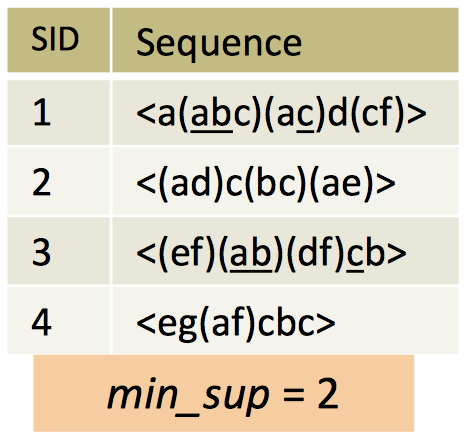
\includegraphics{SPADE_transactions.png}
    \caption{A sequence database}
\end{figure}

\begin{figure}[H]
    \centering
    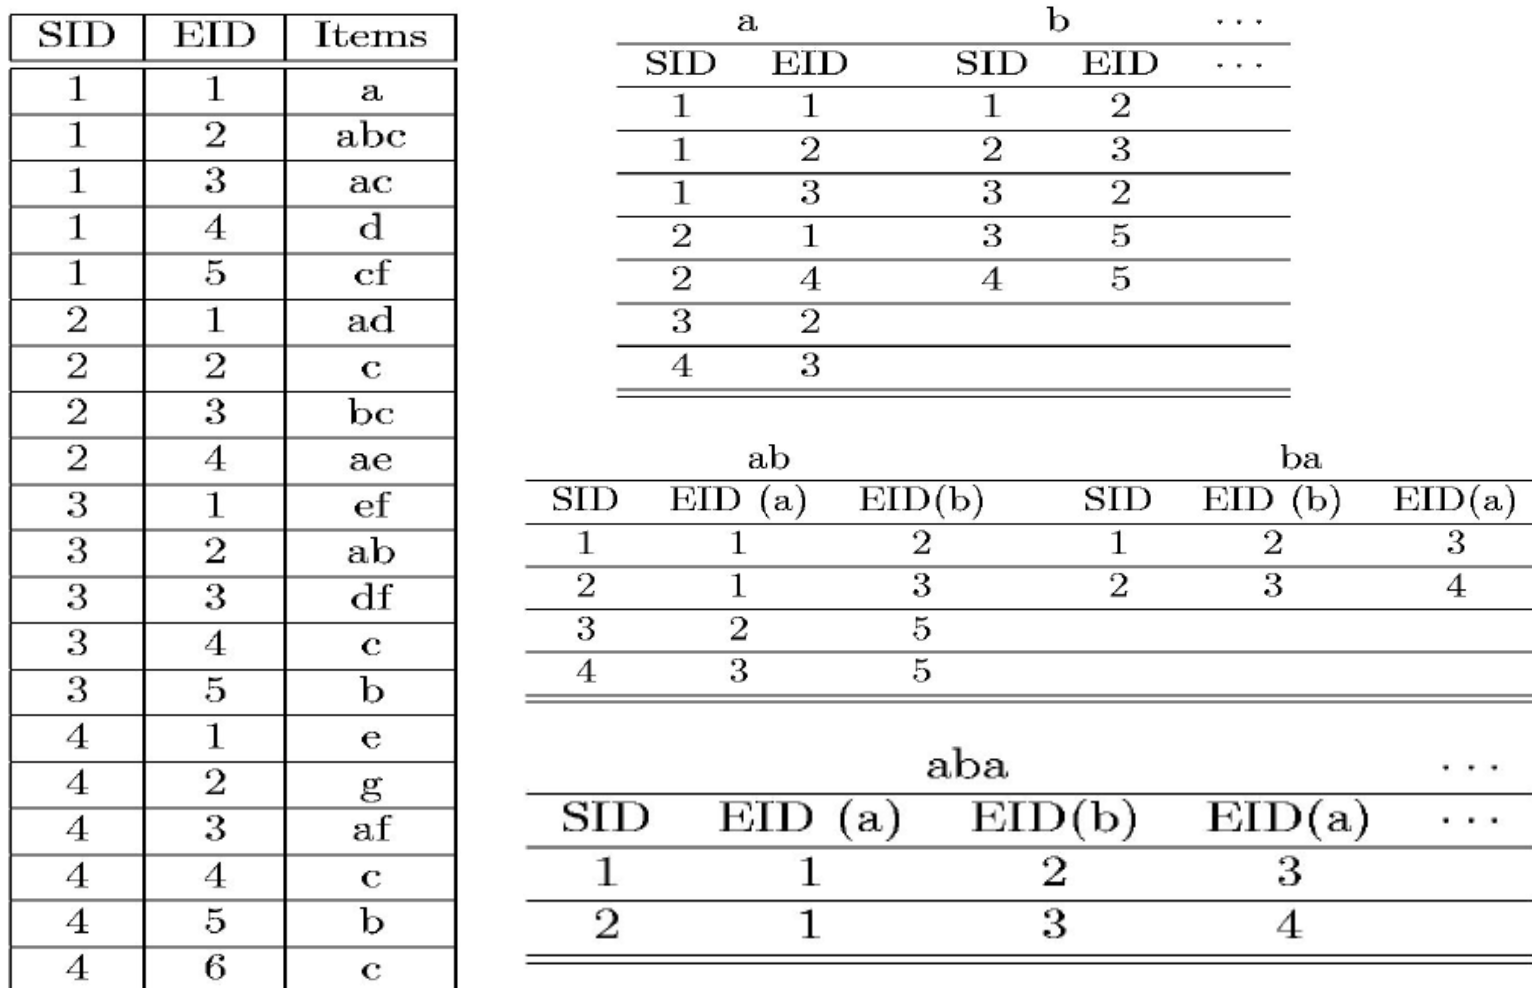
\includegraphics[width=\linewidth]{SPADE_algorithm.png}
    \caption{SPADE algorithm}
\end{figure}

%--
\subsection{PrefixSpan: A Pattern-Growth Approach}
\textbf{PrefixSpan} = Prefix-projected Sequential pattern mining

\begin{figure}[H]
    \centering
    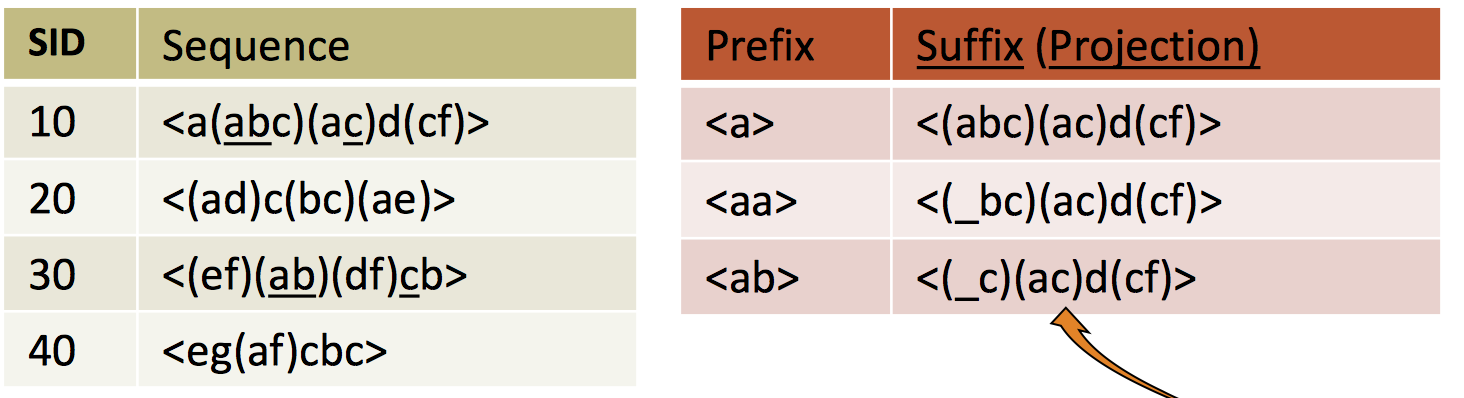
\includegraphics[width=\linewidth]{PrefixSpan.png}
    \caption{SPADE algorithm}
\end{figure}

PrefixSpan Mining: Prefix Projections
\begin{itemize}
\item Step 1: Find length-1 sequential patterns: <a>, <b>, etc.
\item Step 2: Divide search space and mine each projected DB: <a>-projected DB, <b>-projected DB, etc.
\end{itemize}

%--
\subsection{CloSpan: Mining Closed Sequential Patterns}
\begin{definition}
\textbf{A closed sequential pattern $\alpha$}: there exists no superpattern $\beta$ such that $\beta$ and $\alpha$ have the same support:
\end{definition}
\begin{equation*}
CS = \{\alpha \mid \alpha \in FS \textit{ and } \nexists \beta \in FS \textit{, such that } \alpha \subseteq \beta \textit{ and } sup(\alpha) = sup(\beta)\}
\end{equation*}

CloSpan is based on this property: if $s \supset s_1$ then s is closed only if two project DBs have the same size. So redundant search space can be pruned using \textbf{Backward Subpattern} and \textbf{Backward Superpattern} pruning.

\begin{figure}[h]
\centering
\subfigure[backward sub-pattern]{%
  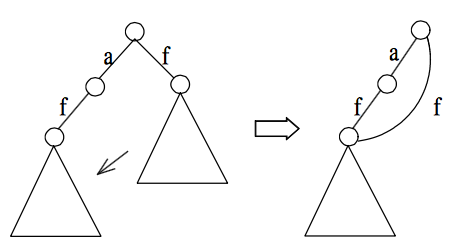
\includegraphics[width=0.32\linewidth, height=0.2\linewidth]{backward_subpattern.png}
  \label{fig:clospan1}}
\quad
\subfigure[backward super-pattern]{%
  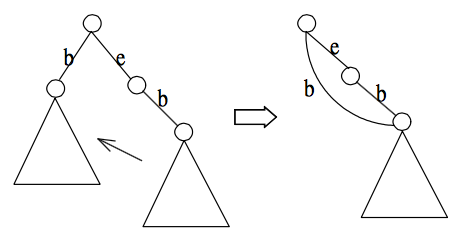
\includegraphics[width=0.32\linewidth, height=0.2\linewidth]{backward_superpattern.png}
  \label{fig:clospan2}}

\caption{CloSpan pruning algorithm}
\label{fig:clospan}
\end{figure}

%--
\subsection{Constraint-Based Sequential-Pattern Mining}

\begin{itemize}
\item \textbf{Anti-monotonic}: If S violates c, the super-sequences of S also violate c
\item \textbf{Monotonic}: If S satisfies c, the super-sequences of S also do so
\item \textbf{Data anti-monotonic}: If a sequence s1 with respect to S violates c3, s1 can be removed
\item \textbf{Succinct}: Enforce constraint c by explicitly manipulating data
\item \textbf{Convertible}: Projection based on the sorted value not in sequence order
\end{itemize}

\subsubsection{Timing-Based Constraints}
\begin{itemize}
\item \textbf{Order constraint}: Some items must happen before the other. Anti-monotonic: constraint-violating sub-patterns pruned
\item \textbf{Min-gap/max-gap constraint}: Confines two elements in a pattern. Succinct: enforced directly during pattern growth
\item \textbf{Max-span constraint}: Maximum allowed time difference between the 1st and the last elements in the pattern. Succinct: enforced directly when the 1st element is determined
\item \textbf{Window size constraint}: Time window allows a group of consecutive elements of a data-sequence to be merged and treated as a single element as long as their timestamps are within the user-specified window-size.
\end{itemize}

%--
\subsection{Recommended Readings}
\begin{itemize}
\item M. N. Garofalakis, R. Rastogi, K. Shim: Mining Sequential Patterns with Regular Expression Constraints. IEEE Trans. Knowl. Data Eng. 14(3), 2002
\item H. Mannila, H. Toivonen, and A. I. Verkamo, “Discovery of frequent episodes in event sequences”, Data Mining and Knowledge Discovery, 1997
\item J. Pei, J. Han, B. Mortazavi-Asl, J. Wang, H. Pinto, Q. Chen, U. Dayal, and M.-C. Hsu, "Mining Sequential Patterns by Pattern-Growth: The PrefixSpan Approach", IEEE TKDE, 16(10), 2004
\item J. Pei, J. Han, and W. Wang, "Constraint-based sequential pattern mining: the pattern-growth methods", J. Int. Inf. Sys., 28(2), 2007
\item R. Srikant and R. Agrawal, “Mining sequential patterns: Generalizations and performance improvements”, EDBT’96
\item X. Yan, J. Han, and R. Afshar, “CloSpan: Mining Closed Sequential Patterns in Large Datasets”, SDM'03
\item M. Zaki, “SPADE: An Efficient Algorithm for Mining Frequent Sequences”, Machine Learning, 2001
\end{itemize}

